\documentclass{article}
\usepackage{tikz}	% (note: AFTER \pdfminorversion)
\usetikzlibrary{matrix}
\usetikzlibrary{fit}
\usetikzlibrary{positioning}


\begin{document}

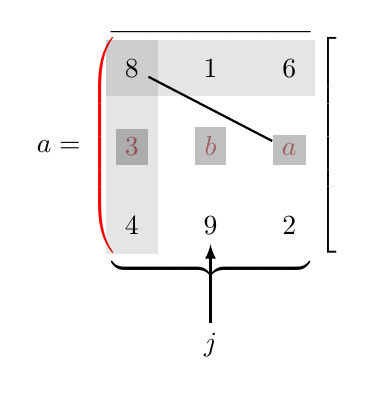
\begin{tikzpicture}
[
	%matrix of nodes/.style			= % CONFLICTS WITH CALLING (nameofthematrix-i-j)
	%{
		%execute at begin cell		= \node\bgroup,
		%execute at end cell		= \egroup;% KEEP THIS ``%''
		%execute at empty cell		= \node{$\star$};%
	%},
	%
	% row 1 | column 2 | every odd row | every even colum
	every even row/.style			=
	{
		nodes						=
		{
			text					= red!50!black,
			fill					= black!50!white,
			fill opacity			= 0.5
		}
	},
	%
	row sep							= {1cm,between origins},
	column sep						= {1cm,between origins},
	%
	% every right delimiter | every above delimiter | every below delimiter
	every left delimiter/.style		= {red,xshift=1ex},
]
	\matrix (mymatrix)
	[
		matrix of math nodes,
		left delimiter			= {(},
		right delimiter			= {[},
		above delimiter			= {|},
		below delimiter			= {\}},
	]
	{
		8 & 1 & 6 \\
		3 & b & a \\
		4 & 9 & 2 \\
	};
	
	\draw [thick] (mymatrix-1-1) -- (mymatrix-2-3);
	
	\node [fill = black, fill opacity = 0.1, fit = (mymatrix-1-1) (mymatrix-1-3)] {};
	\node [fill = black, fill opacity = 0.1, fit = (mymatrix-1-1) (mymatrix-3-1)] {};
	
	\node [left = of mymatrix, anchor = west] {$a = $};
	\node (j) [below = of mymatrix-3-2, anchor = north] {$j$};

	\draw [thick, -latex] (j) -- (mymatrix-3-2);

\end{tikzpicture}

\end{document}
